\documentclass[12pt]{article}
\usepackage{amsfonts, epsfig}
\usepackage[authoryear]{natbib}
\usepackage{graphicx}
\usepackage{fancyhdr}
\pagestyle{fancy}
\lfoot{\texttt{comsm0075.github.io}}
\lhead{IP\&B - 1b\_the\_Bayesian\_brain - Conor}
\rhead{\thepage}
\cfoot{}
\begin{document}

\section*{Sensory processing and probabalistic codes.}

In this section we will begin to explore the idea that the brain
performs Bayesian inference on data. As an example of how this might
apply to perception, we consider the experiment done by Ernst and
Banks \cite{ErnstBanks2002} in which people were asked to judge the
height of a block. The height of the block is $x$ and the subjects
were asked to judge its height under three conditions, visually $v$,
by touch, that is haptically, $h$ and by vision and touch together
$hv$. In the visual trials noise is added using goggles. The set up is
pictured in Fig.~\ref{fig_ernstbanks}


\begin{figure}[htb]
\begin{center}
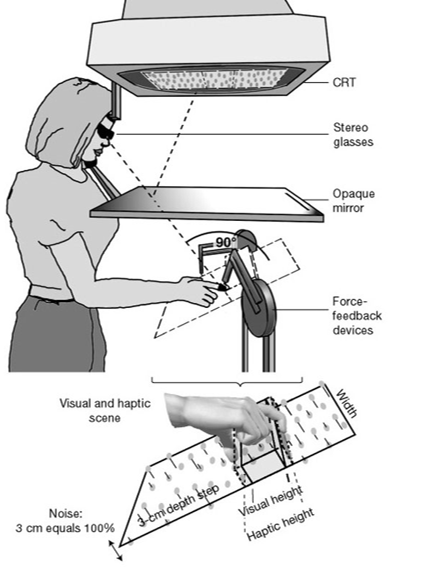
\includegraphics[width=7.5cm]{fig_ernstbanks.png}
\end{center}
\caption{Illustration of the Ernst and Banks experiment. [Pictures
    from Rosalyn Moran who took it from the
    paper]\label{fig_ernstbanks}}
\end{figure}

The joint probability is $p(v,h,x)$, it is assumed that $V$ and $H$
are conditionally independent: 
\begin{equation}
p(v,h|x)=p(v|x)p(h|x)
\end{equation}
In mathematics this would be modelled with a Markov chain
$V\rightarrow X\rightarrow H$, in the world of Bayesian inference this
is illustrated with a \textsl{directed acylcic graph} or \textsl{Bayesian network}:\footnote{Picture from Rosalyn Moran}
\begin{center}
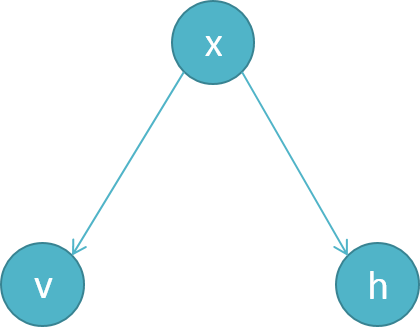
\includegraphics[width=4.5cm]{fig_dag.png}
\end{center}
Either way, the idea is that although there is a relationship between
$V$ and $H$, if the block is big they will both be large, but that
this relationship is only because they are both related to $X$. One consequence of this is
\begin{equation}
p(v,h,x)=p(v|x)p(h|x)p(x)
\end{equation}

We are interested in the posterior judgement of the height of the block:
\begin{equation}
p(x|v,h)=\frac{p(v,h|x)p(x)}{p(v,h)}=\frac{p(v|x)p(h|x)p(x)}{p(v,h)}
\end{equation}
It is assumed that the prior is uniform, so $p(x)$ is constant over some range of possible $x$, so if $x$ is in that range
\begin{equation}
p(x|v,h)\propto \frac{p(v|x)p(h|x)}{p(v,h)}
\end{equation}
The value of $x$ that maximizes this is called the \textsl{maximum a posteriori}.

Now the purpose of the Ernst and Banks experiment is to study sensory
fusion, the fusing of two noisy pieces of evidence. Bayesian analyses
is used to show the optimal fusing of the data, this is what we will
derive now. This is then compared to data to show that the brain
approaches the problem in an optimal way. 

It is assumed that the haptic and visual channels have independent
Gaussian noise around the true value, that is
$\mathcal{N}(x,\sigma_v^2)$ and $\mathcal{N}(x,\sigma_h^2)$
respectively, so
\begin{equation}
p(v|x)=\frac{1}{\sqrt{2\pi\sigma_v^2}}e^{-\frac{(v-x)^2}{2\sigma_v^2}}
\end{equation}
and 
\begin{equation}
p(h|x)=\frac{1}{\sqrt{2\pi\sigma_v^2}}e^{-\frac{(h-x)^2}{2\sigma_h^2}}
\end{equation}
and we ignore the normalizing factor $p(v,h)$ since it is independent of $x$, then
\begin{equation}
p(x|v,h)\propto p(v|x)p(h|x)
\end{equation}

Now if we multiply out the two Gaussians the exponent is
\begin{equation}
-\frac{(h-x)^2}{2\sigma_h^2}-\frac{(v-x)^2}{2\sigma_v^2}=-\left(\frac{1}{2\sigma_h^2}+\frac{1}{2\sigma_v^2}\right)x^2+\left(\frac{h}{\sigma_h^2}+\frac{v}{\sigma_v^2}\right)x+\mbox{other stuff}
\end{equation}
so if we define $\sigma$ by
\begin{equation}
\frac{1}{\sigma^2}=\frac{1}{\sigma_v^2}+\frac{1}{\sigma_h^2}
\end{equation}
and $\bar{x}$ by
\begin{equation}
\bar{x}=\frac{\sigma^2}{\sigma_v^2}v+\frac{\sigma^2}{\sigma_h^2}h
\end{equation}
this gives
\begin{equation}
-\frac{(h-x)^2}{2\sigma_h^2}-\frac{(v-x)^2}{2\sigma_v^2}=-\frac{(x-\bar{x})^2}{2\sigma^2}+\mbox{other stuff}
\end{equation}

In other words, the optimal guess for $x$ is the variance weighted
measurements of $v$ and $h$; the factors $\sigma^2/\sigma_v^2$ and
$\sigma^2/\sigma_h^2$ quantify how much the variability of $v$ and $h$
contribute to the variability of $\bar{x}$, and the more they
contribute, the lower the weighting is given to the measurement. This
is summarized by writing $\lambda_v=\sigma^2/\sigma_v^2$ and
$\lambda_h=\sigma^2/\sigma_h^2$, so
\begin{equation}
\lambda_v+\lambda_h=\frac{\sigma^2}{\sigma_v^2}+\frac{\sigma^2}{\sigma_h^2}=\frac{1}{1/\sigma_v^2+1/\sigma_h^2}\left(\frac{1}{\sigma_v^2}+\frac{1}{\sigma_h^2}\right)=1
\end{equation}
so $\lambda_v$ and $\lambda_h$ are the visual and haptic weights.

In the actual experiment the visual noise is changed, allowing the
experimenters to manipulate the two weights. They then do multiple
experiments where they ask the subjects to decide which of two blocks
is larger and manage through a regression analysis to decide how the
subjects are weighting the two pieces of evidence. In other words it is assumed that the subjects are combining the haptic and visual estimates
\begin{equation}
\xi=\mu_v v+\mu_h h
\end{equation}
where $\xi$ is the subjects estimate of $x$ and $\mu_v$ and $\mu_h$
are some weighting factors to be estimated from the behavioural data
by regression; for details see the paper. They then compare the
measured weightings, $\mu_v$ and $\mu_h$, to those estimated by the
optimal Bayesian model, that is $\lambda_v$ and $\lambda_h$. The
result is shown in Fig.~\ref{fig_weights} and demonstrate Bayesian
optimal perception in this aspect of human sensory fusion.


\begin{figure}[htb]
\begin{center}
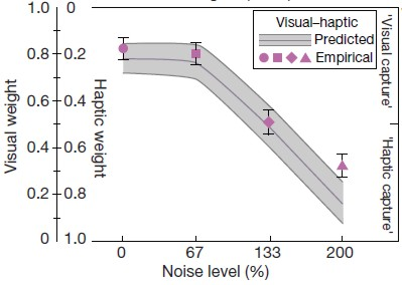
\includegraphics[width=7.5cm]{fig_weights.png}
\end{center}
\caption{Results of the Ernst and Banks experiment. As the weights are
  changed by manipulating the visual noise by adjusting the goggles,
  the weighting of how the visual and haptic information are fused
  should change according to the grey line; by a clever set of tests
  it is possible to estimate the true weightings used by the subjects,
  these are the red features. The match is very good.[Pictures from
    Rosalyn Moran who took it from the paper]\label{fig_weights}}
\end{figure}

\bibliographystyle{apalike}
\bibliography{../../source/bibliography}{}

\end{document}

